\section{Versuchsauswertung}

\subsection{Speicher A}

\subsubsection{UA-Wert Plattenwärmeübertrager}
Zur Bestimmung des UA-Wertes wurden die zu Beginn der Speicherbeladung aufgenommenen Messdaten verwendet. Diese sind in Abbildung \ref{fig:extWT} gezeigt. Für die Berechnung wurde der Stationäre Temperaturverlauf zwischen den Scans 150 und 270 gemittelt. Zusätzlich wurde der Volumenstrom des orangenen MIDs zum gegeben Zeitraum erfasst. 

\begin{figure}[H]
	\centering
	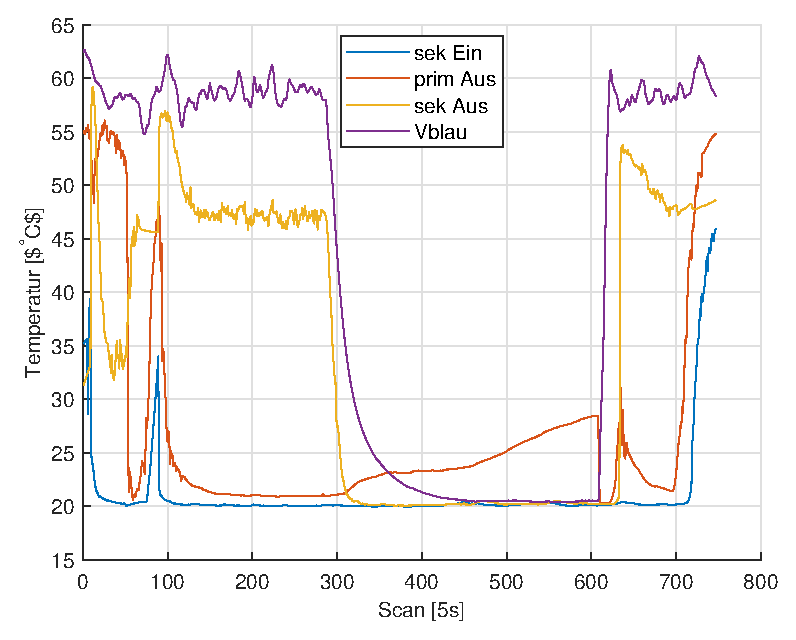
\includegraphics[width=0.8\textwidth]{../DATA/PlattenWT_A.eps}
	\caption[Temperaturverläufe des Platten-WÜT]{Temperaturverläufe des Platten-WÜT}
	\label{fig:extWT}
\end{figure}

Die benötigten Temperaturen sind in Tabelle \ref{tab:extWT} zusammengefasst. Der Volumenstrom beträgt 0,0874 $\pm$1,8614e-04 $\frac{m^3}{h}$.

\begin{center}
	\begin{tabular}{l|c}
		\label{tab:extWT}
		
		\textbf{Messwert} & \textbf{Mittelwert} [${\celsius}$] \\
		\hline
	$T_{sek,ein}$ & 20,0646 $\pm$0,0397\\
	$T_{sek,aus}$ & 47,1604 $\pm$0,5687\\
	$T_{prim,ein}$ & 58,8494 $\pm$0,8431\\
	$T_{prim,aus}$ & 21,0185 $\pm$0,0965\\
	
	\end{tabular}
\end{center}
Die Berechnung erfolgt gemäß Gleichung \ref{eq:QextWT} bis \ref{eq:UAext}. Näherungsweise wurden eine Wasserdichte von \SI{1000}{\kilogram\per\cubic\meter} und eine Wärmekapazität von \SI{4190}{\joule\per\kilogram\kelvin} angenommen.
\begin{equation}
	\label{eq:QextWT}
	\dot Q_{WÜT} = \rho_{w} * \dot V_{MID,orange} * c_{p,w} * (T_{prim,ein}-T_{prim,aus}) = \SI{3850}{\watt}
\end{equation}

\begin{center}
	\begin{small}
	$\dot Q_{WÜT}$:Wärmestrom am WÜT,	
	$\rho_{w}$:	Dichte von Wasser,
	$c_{p,w}$: Wärmekapazität von Wasser
	\end{small}
\end{center}

\begin{equation}
	\label{eq:DeltaTm}
	\Delta T_{m} = \frac{|\Delta T_{0} - \Delta T_{1}|}{ln(\frac{\Delta T_{0}}{\Delta T_{1}})} = \SI{4,2840}{\kelvin}
\end{equation}
\begin{center}
	\begin{small}
		$\Delta T_{m}$: Mittlere Temperaturdifferenz
	\end{small}
\end{center}

mit
\begin{equation}
	\label{eq:DeltaT0}
	\Delta T_{0} = T_{prim,ein} - T_{sek,aus}
\end{equation}

\begin{equation}
	\label{eq:DeltaT1}
	\Delta T_{1} = T_{prim,aus} - T_{sek,ein}
\end{equation}
Der UA Wert ergibt sich aus dem Quotienten von Gleichung \ref{eq:QextWT} und \ref{eq:DeltaTm}.
\begin{equation}
	\label{eq:UAext}
	UA_{WÜT} = \frac{\dot Q_{WÜT}}{\Delta T_{m}} = \SI{898,7}{\watt\per\kelvin}
\end{equation}

\subsubsection{Füllvorgang}
Bei der Befüllung wurde der Temperaturverlauf an der Messlanze beobachtet und aufgezeichnet. Abbildung \ref{fig:SpAfill} zeigt den zugehörigen Datensatz mit den verschiedenen Messpunkten.

\begin{figure}[H]
	\centering
	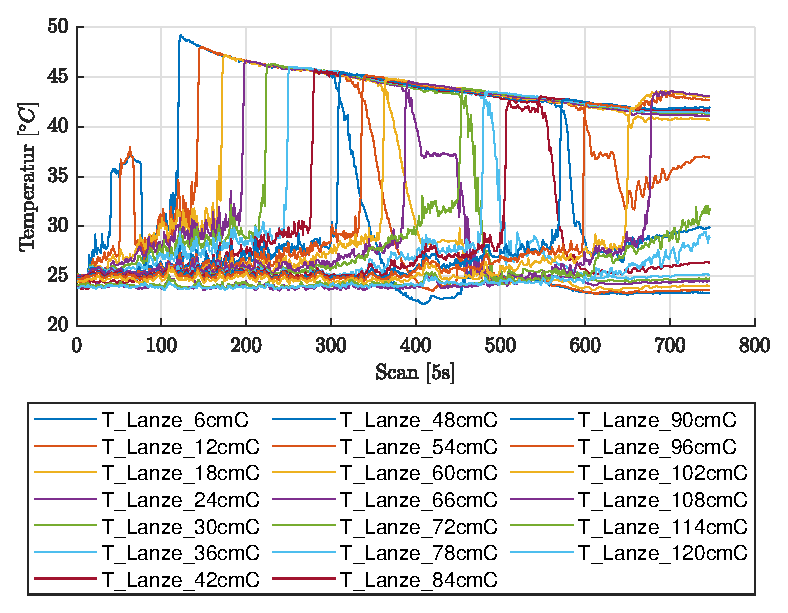
\includegraphics[width=0.8\textwidth]{../DATA/SpA_Lanzen.eps}
	\caption[Temperaturverlauf Speicher A]{Temperaturverlauf der Befüllung von Speicher A}
	\label{fig:SpAfill}
\end{figure}

